\documentclass[12pt]{article}
\usepackage{tikz}
\usepackage{amssymb}
\usepackage{amsmath}

\begin{document}

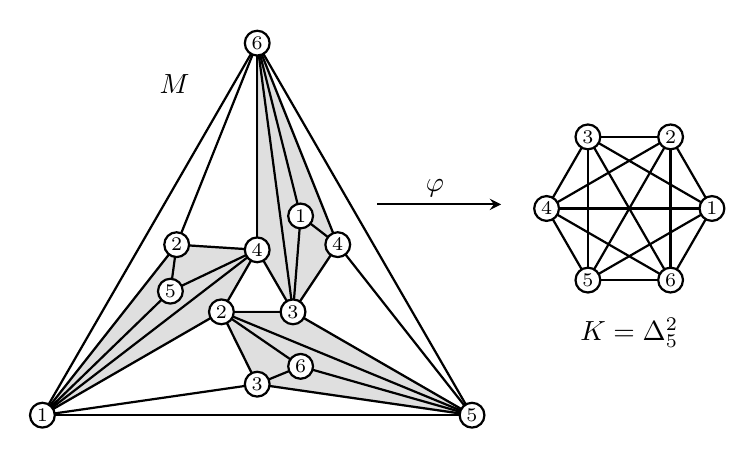
\begin{tikzpicture}[scale=0.525,style=thick]
\def\h{6}
\def\hh{1}
\def\hhh{2.25}
\def\vr{0.3}
\def\sh{4.5}
\def\tr{2.1} %Tetra radius
\draw [color=lightgray, fill=lightgray, fill opacity=0.5] (90:\h)--(30:\hhh)--(330:\hh)--(90:\hh)--(90:\h);
\draw [color=lightgray, fill=lightgray, fill opacity=0.5] (90+120:\h)--(30+120:\hhh)--(330+120:\hh)--(90+120:\hh)--(90+120:\h);
\draw [color=lightgray, fill=lightgray, fill opacity=0.5] (90-120:\h)--(30-120:\hhh)--(330-120:\hh)--(90-120:\hh)--(90-120:\h);
\foreach \x  in {90,210,330} \draw (\x:\hh)--(\x+120:\hh);
\foreach \x  in {90,210,330} \draw (\x:\h)--(\x+120:\h);
\foreach \x  in {-90,30,150} \draw (\x:\hhh)--(\x+60:\h);
\foreach \x  in {-90,30,150} \draw (\x:\hhh)--(\x-60:\h);
\foreach \x  in {-90,30,150} \draw (\x:\hhh)--(\x-60:\hh);
\foreach \x  in {90,210,330} \draw (\x:\hh)--(\x+120:\h);
\foreach \x  in {90,210,330} \draw (\x:\hh)--(\x:\h);
\foreach \x  in {180,60,300} \draw (\x-30:\hhh)--(\x:\tr)--(\x+30:\h);
\foreach \x  in {90,210,330} \draw (\x:\hh)--(\x+90:\tr);
\foreach \x  in {90,210,330} \draw (\x:\h) [fill=white] circle (\vr);
\foreach \x  in {90,210,330} \draw (\x:\hh) [fill=white] circle (\vr);
\foreach \x  in {-90,30,150} \draw (\x:\hhh) [fill=white] circle (\vr);
\foreach \x  in {180,60,300} \draw (\x:\tr) [fill=white] circle (\vr);
\draw (90:\h) node {\scriptsize 6};
\draw (210:\h) node {\scriptsize 1};
\draw (330:\h) node {\scriptsize 5};
\draw (90:\hh) node {\scriptsize 4};
\draw (210:\hh) node {\scriptsize 2};
\draw (330:\hh) node {\scriptsize 3};
\draw (-90:\hhh) node {\scriptsize 3};
\draw (30:\hhh) node {\scriptsize 4};
\draw (150:\hhh) node {\scriptsize 2};
\draw (180:\tr) node {\scriptsize 5};
\draw (60:\tr) node {\scriptsize 1};
\draw (300:\tr) node {\scriptsize 6};
\draw [->,>=stealth] (2.9,2.1)--+(3,0);
\foreach \x in {1,2,3,4,5,6} \draw (9,2) +(\x*60-60:2)--+(\x*60:2);
\foreach \x in {1,2,3,4,5,6} \draw (9,2) +(\x*60-60:2)--+(\x*60+60:2);
\foreach \x in {2,4,6} \draw (9,2) +(\x*60:2)--+(\x*60+180:2);
\foreach \x in {1,2,3,4,5,6} \draw (9,2) +(\x*60-60:2) [fill=white] circle (\vr) node {\scriptsize $\x$};
\draw (-2,5) node {$M$};
\draw (9,-1) node {$K=\Delta_5^{2}$};
\draw (4.3,2.5) node {$\varphi$};
\end{tikzpicture}

\end{document}